\documentclass[letterpaper]{book}

\usepackage{amssymb}
\usepackage{amsthm}
\usepackage{amsmath}
\usepackage[left=1in, right=1in, top=1in, bottom=1in]{geometry}
\usepackage{graphicx}
\usepackage[parfill]{parskip}
\usepackage{hyperref} 
\usepackage{titlesec}
\usepackage{mdframed}
\usepackage{enumitem}

\newcommand{\ZZ}{\mathbb{Z}}
\newcommand{\NN}{\mathbb{N}}
\newcommand{\QQ}{\mathbb{Q}}

\newcommand{\ord}{\operatorname{ord}}
\newcommand{\ind}{\operatorname{ind}}

\newtheorem{lemma}{Lemma}
\newtheorem{sublemma}{Lemma}[lemma]
\newtheorem{theorem}{Theorem}[section]
\newtheorem{corollary}{Corollary}[section]
\newtheorem{definition}{Definition}[section]
\newtheorem{proposition}{Proposition}[section]
\newtheorem{example}{Example}[theorem]

\titleformat{\chapter}[display]
    {\normalfont\bfseries}{}{0pt}{\LARGE}

\title{M 328K}
\author{Katherine Ho}
\date{}

\begin{document}
\maketitle
\tableofcontents
\chapter{Lecture 1}
\date{August 27, 2024}

\section{Open Problems}
    \begin{itemize}
        \item Twin Primes Conjecture: Do there exist infinitely many pairs of primes 
        that are 2 apart?
        \item Collatz Conjecture, 3n+1 Problem - Does this process eventually stop for all n?
        \item Fermat's Last Theorem: The equation $x^n+y^n=z^n$ has no (non-trivial)
        integer solution when $n\geq 3$. \\
            Note: When $n=2$, there are infinite solutions (Pythagorean triples)
    \end{itemize}

\section{Notation}
    \begin{itemize}
        \item Natural numbers: $\mathbb{N} = \{1,2,3,4,\dots\}$
        \item Integers: $\mathbb{Z} = \{\dots,-2,-1,0,1,2,\dots\}$
        \item Rational Numbers: $\mathbb{Q} = \{\frac{a}{b}|a,b\in\mathbb{Z}, b\neq 0\}$
    \end{itemize}

\section{Divisibility}
    \begin{definition}
        Let $n,m\in\mathbb{Z}$. We say that $n$ divides $m$ and write $n|m$ if there exists
        an integer $k$ such that $m=nk$. 
        \[ \text{Ex: } 2|4, 5|-5, 3|0, 0|0\]
        If n does not divide m: $n\nmid m$
        \[ \text{Ex: } 2\nmid 3, 0\nmid 5\]
    \end{definition}

    \begin{theorem}
        For $a,b,c\in\mathbb{Z}$, the following hold:
        \begin{enumerate}
            \item $a|0$, $1|a$, $a|a$
            \item $a|1$ iff $a=\pm b$
            \item If $a|b$ and $c|d$ then $ac|bd$
            \item If $a|b$ and $b|c$ then $a|c$
            \item $a|b$ and $b|a$ iff $a=\pm b$
            \item If $a|b$ and $b\neq 0$, then $|a|\leq |b|$
            \item If $a|b$ and $a|c$, then $a|(bx+cy)$ for $x,y\in\mathbb{Z}$ \\
                Ex. If b, c are even, then (any multiple of b) +
                (any multiple of c) is even.
        \end{enumerate}

        \begin{proof} [Proof (2)]
            First, assume $a|1$. By definition, there exists an integer k 
            such that $1=ak$. \\ Note: $k\neq 0$ and $a\neq 0$, so
            \[ |ak|=|a||k| \geq |a| \text{ since } |k| \geq 1 \]
            Thus, $1=|ak|\geq |a|$. \\
            Also, $|a|\geq 1$ since $a\neq 0$ and $a\in\mathbb{Z}$.
            Thus, $|a|=1$ which is equivalent to $a=\pm 1$. \\\\
            Next, assume $a=\pm 1$.
            \begin{itemize}
                \item If $a=1$: $a|1$ since $1=a\cdot 1$
                \item If $a=-1$: $1=a\cdot -1$
            \end{itemize}
            In both cases, $a|1$ as desired.
        \end{proof}

        \begin{proof} [Proof (4)]
            Assume $a|b$ and $b|c$. \\
            By definition, there exist integers i and j such that 
            $b=a\cdot i$ and $c=b\cdot j$. \\
            Then, $c=(a\cdot i)\cdot j=a(ij)$. \\
            So, $a|c$ by definition.
        \end{proof}
    \end{theorem}

\section{The Division Algorithm}
    \begin{theorem}
        Given integers a and b with $b\neq 0$, there exist unique integers q and r such that
        \[ a=bq+r,\ 0\leq r\leq |b| \]
    \end{theorem}

\chapter{Lecture 2}
\date{August 29,2024}

\section{Proof by Contradiction}
    To prove a statement p, assume p is false and derive a contradiction.
    \begin{theorem}
        $\sqrt{2}$ is irrational.
        \begin{proof}
            Assume $\sqrt{2}$ is rational.
            So there exist integers a,b s.t. 
            \[
                \sqrt{2} = \frac{a}{b}, \text{ where a and b have no common factors.}
            \]
            Thus $2b^2=a^2$. ie. $2|a^2$.
            Hence also $2|a$. By definition, we can write $a=2k$ for some $k\in\mathbb{Z}$.
            Then,
            \begin{align*}
                2b^2 &= (2k)^2 = 4k^2 \\
                b^2 &= 2k^2
            \end{align*}
            So $2|b^2$, hence $2|b$.
            Thus, 2 is a common factor of a and b, a contradiction. \\
            Therefore, $\sqrt{2}$ is irrational.
        \end{proof}
    \end{theorem}

\section{Proof by Induction}
    Use to prove an infinite number of statements. 
    Ex: Prove that the sum of the first n odd integers is $n^2$. \\
    Strategy: 
    \begin{itemize}
        \item Prove base case(s) n=0,1
        \item Prove that if the statement is true for n, then it is true for n+1
    \end{itemize}

    \begin{proof} [Proof by Induction]
        Base case: For n=1, the sum of the first n positive odd integers is 1, which is $n^2$. \\
        Induction step: Assume that the sum of the first n odd integers is $n^2$.
        Consider the sum of the first n+1 odd integers.
        \[
            \sum_{k=1}^{n+1}2k-1 = 1+3+5+\dots+2n-1+2(n+1)-1
        \]
        By the induction hypothesis, we have
        \begin{align*}
            \sum_{k=1}^{n+1}2k-1 &= n^2+2(n+1)-1 \\
            &= n^2 + 2n + 2 - 1 \\
            &= n^2 + 2n + 1 \\
            &= (n+1)^2, \text{ as desired}
        \end{align*}
    \end{proof}

    \begin{theorem}
        For $n\geq 1, \frac{d}{dx}x^n = nx^{n-1}$.
        \begin{proof} [Proof by Induction]
            Base case: n=1. $\frac{d}{dx}x^1=1=1\cdot x^0$. \\
            Induction step: Assume $\frac{d}{dx}x^n = nx^{n-1}$ is true for some $n>1$. 
            Using the power rule, we have
            \begin{align*}
                \frac{d}{dx}x^{n+1} &= x(nx^{n-1})+x^n \\
                &= n\cdot x^{1+(n-1)}+x^n \\
                &= x^n(n+1) \\
                &= (n+1)x^n, \text{ as desired.}
            \end{align*}
        \end{proof}
    \end{theorem}

\section{Well Ordering Principle (WOP)}
    Every nonempty subset of $\mathbb{N}$ has a smallest element.
    \begin{theorem} [Division Algorithm]
        For any $a,b\in\mathbb{Z}$ with $b\neq 0$, there exist unique integers q,s s.t.
        $a=bq+r, 0\leq r<|b|$.
        \begin{proof}
            Consider the set 
            \[ S=\{a-bx|x\in\mathbb{Z}, a-bx\geq 0\} \]
            For simplicity, assume $b>0$. Note that S is nonempty since for $x=-|a|$, we have
            \begin{align*}
                a-bx = a-b-(-|a|) &= a+b|a| \\
                & \geq a+|a| \\
                & \geq 0
            \end{align*}
            So, $a-bx\in S$. \\\\
            By WOP, S has a smallest element r. Call the corresponding value of x by q. \\
            So $r=a-bq \Leftrightarrow a=bq+r$. \\\\
            Now, we want to show that $0\leq r\leq |b|\ (=b)$ since $b>0$. \\
            By way of contradiction, assume $r\geq b$. 
            Consider
            \begin{align*}
                a-b(q+1) &= a-bq-b \\
                &= r-b \\
                & \geq 0
            \end{align*}
            Thus, $a-b(q+1)$ is an element of S that is smaller than r, a contradiction. \\\\
            Suppose there exist $q_1,r_1,q_2,r_2\in\mathbb{Z}$ such that 
            \[ a=bq_1+r_1 = bq_2+r_2 \]
            where $0\leq r_1,r_2 < b$ (still assuming $b > 0$).
            We want to show $q_1=q_2, r_1=r_2$.
            We have 
            \begin{align*}
                bq_1-bq_2 &= r_1-r_2 \\
                b(q_1-q_2) &= r_1-r_2 \\
                b|q_1-q_2| &= |r_1-r_2| < b
            \end{align*}
            But $b|q_1-q_2| < b$ implies (since $b > 0$) that 
            \[ 0\leq |q_1-q_2|<1 \]
            So, $q_1-q_2$ since $q_1,q_2\in\mathbb{Z}$
            Thus also $r_1=r_2$.
        \end{proof}
    Note: The division algorithm lets us make statements like "Every integer can be 
    expressed uniquely in the form $4k, 4k+1, 4k+2, or 4k+3$"
    \end{theorem}

    \begin{theorem}
        The square of every odd integer is of the form $8k+1$.
        \begin{proof}
            By the division algorithm, any odd integer n is of the form $n=4k+1$ or 
            $4k+3$. \\
            In the 1st case,
            \begin{align*}
                n^2 &= (4k+1)^2 \\
                &= 16k^2+8k+1 \\
                &= 8(2k^2+3k+1)
            \end{align*}
            In the 2nd case,
            \begin{align*}
                n^2 &=(4k+3)^2 \\
                &= 16k^2+24k+9 \\
                &= 8(2k^2+3k+1)+1
            \end{align*}
        \end{proof}
    \end{theorem}

    \begin{definition}
        For $a,b,c\in\mathbb{Z}$, if $c|a$ and $c|b$, we say that c is a common divisor 
        and has the property that for any other common c of a and b that $d\geq c$, 
        we call d the greatest common divisor of a and b, and write $d=\gcd(a,b)$.
    \end{definition}

\documentclass[letterpaper]{article}

\usepackage{amssymb}
\usepackage{amsthm}
\usepackage{amsmath}
\usepackage[left=1in, right=1in, top=1in, bottom=1in]{geometry}

\newtheorem{lemma}{Lemma}
\newtheorem{sublemma}{Lemma}[lemma]
\newtheorem{theorem}{Theorem}[section]
\newtheorem{corollary}{Corollary}[section]
\newtheorem{definition}{Definition}[section]
\newtheorem{example}{Example}[theorem]

\title{M 328K: Lecture 3}
\author{Katherine Ho}
\date\today

\begin{document}
\maketitle

\section{Problem}
    If a rooster is worth 5 coins, a hen 3 coins, and 3 chicks together 1 coin,
    how many roosters, hens, and chicks, totaling 100, can be bought for 100 coins?
    \begin{align*}
        x & = \# roosters \\
        y & = \# hens \\
        z & = \# chicks 
    \end{align*}
    \begin{align*}
        x+y+z & = 100 \\
        5x + 3y + \frac{1}{3}z & = 100
    \end{align*}
    \begin{center}
        \underline{Diophantine Equations}
    \end{center}
    \begin{align*}
        x^n+y^n & = z^n \\
        x^2+y^2+z^2+w^2 & = n
    \end{align*}

\section{Bezout's Theorem}
    Let $a,b\in\mathbb{Z}$ (not both zero). The gcd of $a$ and $b$ is the smallest
    positive integer $d$ that can be written as $ax+by=d, x,y\in\mathbb{Z}$.
    \begin{proof}
        Let $S = \{ax+by>0 | x,y\in\mathbb{Z}\}$. 
        Note that S is nonempty since for $x=a$, $y=b$ we have $ax+by= a^2+b^2>0$.
        By WOP, S has a smallest element, call it d. WTS:
        \begin{enumerate}
            \item $d|a$, $d|b$
            \item if $c|a$, $c|b$, then $c\leq d$
        \end{enumerate}
        To show $d|a$, apply the division algo to obtain $a=d\cdot q + r, 0\leq r<d$. \\
        Writing $d=ax_0 + by_0$ for $x_0,y_0\in\mathbb{Z}$, we have
        \begin{align*}
            r & = a-d\cdot y \\
            r & = a(ax_0 + by_0)\cdot q \\
            r & = a(1-x_0q) + b(-y_0q)
        \end{align*}
        Hence, if $r>0$ then $r\in S$ which is smaller than d, contradicting d being
        the smallest element. Then, $r=0$ and $d|a$. (Same argument for $d|b$). \\
        Now suppose that $c\in\mathbb{Z}$ such that $c|a$ and $c|b$. Recall that if x and y
        are integers, then $c|(cx+by)$. Hence, $c|(ax_0+by_0) <=> c|d$. 
        Then $c\leq |d| = d$.
        Therefore, $d=\gcd(a,b)$.
    \end{proof}
    \begin{corollary}
        Every common divisor of $a$ and $b$ divides $\gcd(a,b)$.
    \end{corollary}
    \begin{corollary}
        The linear Diophantine equation $ax+by=c$ has a solution iff $d|c$.
    \end{corollary}
    \begin{proof}
        First assume that $ax+by=c$ has a solution: $c=ax_0+by_0$. 
        Since $d|a$, and $d|b$, we have $d|(ax_0+by_0)$. \\
        One the other hand, suppose $d|c$. By definition, $c=d|k$ for some k. \\
        By Bezout's theorem, we can write 
        \[
            d=ax+by \text{ for some } x,y\in\mathbb{Z}
        \]
        Then,
        \begin{align*}
            d\cdot k & = a(x\cdot k) + b(y \cdot k) \\
            c & = a(x\cdot k)+b(y\cdot k)
        \end{align*}
        So c is an integer linear combo $a < b$ as desired.
    \end{proof}

    \begin{definition}
        We say that integers a and b (not both zero) are relatively prime or coprime if
        \[
            \gcd(a,b) = 1
        \]
    \end{definition}
    \begin{corollary}
        Integers a and b are relatively prime iff there exist $x,y\in\mathbb{Z}$ such that
        $ax+by=1$.
    \end{corollary}
    \begin{corollary}
        If a, b are coprime, then $ax+by=c$ has a solution for any $c\in\mathbb{Z}$.
    \end{corollary}

\section{Euclidean Algorithm}
    \begin{enumerate}
        \item Start with (a,b) (assume $|a|\geq |b|$)
        \item Apply DA: $a = bq+r, 0 \leq r < |b|$
        \item If $r=0$, then $b|a$ and $\gcd(a,b) = |b|$.
        \item Otherwise, replace $(a,b)$ with $(b,r)$.
        \item Repeat.
        \item The final nonzero r is gcd.
    \end{enumerate}
    \begin{example}
        $\gcd(12378,3054)$
        \begin{align*}
            12378 & = 3054\cdot 4 + 162 \\
            3054 & = 162\cdot 18 + 138 \\
            162 & = 138\cdot 1 + 24 \\
            138 & = 24\cdot 5 + 18 \\
            24 & = 18\cdot 1 + 6 \\
            18 & = 6\cdot 3 + 0 
        \end{align*}
        \begin{center}
            $\gcd = 6$
        \end{center}
        Note: if you allow for negative remainders, that can be more efficient.
        \begin{align*}
            3054 & = 162\cdot 19 - 24 \\
            162 & = (-24)(-7) - 6 \\
            -24 & = (-6)(4) + 0
        \end{align*}
    \end{example}

    \begin{example}
        Solve $1237x+3054y = 6$ via "Extended Euclidean Algorithm".
        \begin{align*}
            6 & = 24-18\cdot 1 \\
            & = 24-(138-24*5) \\
            & = 24\cdot 6 - 138 \\
            & = (162-138)\cdot 6 - 138 \\
            & = 162\cdot 6 - 138\cdot 7 \\
            & = 162\cdot 6 - (3054-162\cdot 18) \cdot 7 \\
            & = (12378-3054\cdot 4)\cdot 6 - (3054-(12378-3054))\cdot 7
        \end{align*}
    \end{example}
        
    \begin{example}
        Solve
        \begin{align*}
            x+y+z & = 100 \\
            5x+3y+\frac{1}{3}z & = 100 \\
        \end{align*}
        Using $z=100-x-y$, we have $7x+4y = 100$. \\
        Note: $7(-1) + 4(2) = 1$. \\
        So $7(-100) + 4(200) = 100$
        
        \begin{align*}
            7 & = 4\cdot 1 + 3 \\
            4 & = 3\cdot 1 + 1 \\
            1 & = 4-3 \\
            1 & = 4 - (7-4) \\
            1 & = -7 + 4(2)
        \end{align*}
    \end{example}

    \begin{theorem}
        If $ax+by=c$ has a solution $x_0,y_0\in\mathbb{Z}$. Then any other solution
        $x,y\in\mathbb{Z}$ is given by 
        \[
            x=x_0 + \frac{b}{d}k, y = y_0-\frac{a}{d}k        
        \]
        where $k\in\mathbb{Z}$ and $d=\gcd(a,b)$. \\
        If $x,y,z >0$, then k must satisfy
        \[
            \frac{200}{7} > k > 25
        \]
        So
        \[
            k = 26,27,28 \text{, so the only solutions are}
        \]
        \begin{align*}
            x & = 4, y = 18, z = 78 \\
            x & = 8, y = 11, z = 81 \\
            x & = 12, y = -1, z = 89
        \end{align*}
        
    \end{theorem}


\end{document}

\documentclass[letterpaper]{article}

\usepackage{amssymb}
\usepackage{amsthm}
\usepackage{amsmath}
\usepackage[left=1in, right=1in, top=1in, bottom=1in]{geometry}

\newtheorem{lemma}{Lemma}
\newtheorem{sublemma}{Lemma}[lemma]
\newtheorem{theorem}{Theorem}[section]
\newtheorem{corollary}{Corollary}[theorem]
\newtheorem{definition}{Definition}[section]
\newtheorem{example}{Example}[theorem]

\title{M 328K: Lecture 4}
\author{Katherine Ho}
\date\today

\begin{document}
\maketitle

\section{}
    \begin{enumerate}
        \item If $a|c$ and $b|c$, must $ab|c$? \\
        False: $a=b=c=2$, $2|2$, $2|2$ but $4\nmid 2$ 
        \item If $a|bc$ and $a\nmid b$, must $a|c$? \\
        False: $a=4, b=c=2$
    \end{enumerate}
    
    But\dots Proposition: Let $a,b,c\in\mathbb{Z}$
    \begin{enumerate}
        \item If $a|c, b|c$ and $\gcd(a,b)=1$, then $ab|c$.
        \begin{proof}
            By Bezout, there exist integers $x,y$ s.t. $ax+by=1$. 
            Then, $acx+bcy = c$. \\
            By definition, there exist $r,s\in\mathbb{Z}$ s.t. $c=ar=bs$. 
            Thus, 
            \begin{align*}
                a(bs)x + b(ar)y &= c \\
                ab(sx+ry) &= c
            \end{align*}
            So, $ab|c$.
        \end{proof}

        \item If $a|bc$, and $\gcd(a,b)=1$, then $a|c$. (Euclid's Lemma)
        \begin{proof}
            Again, there exist $x,y\in\mathbb{Z}$ s.t. $ax+by=1$.
            Then $acx+bcy=c$. \\
            Since $a|bc$, we have $bc=ar$ for some $r\in\mathbb{Z}$.
            Hence 
            \begin{align*}
                acx+ary &= c \\
                a(cx+ry) &= c
            \end{align*}
            So, $a|c$ as desired.
        \end{proof}
        
    \end{enumerate}

\section{Prime Numbers}
    \begin{definition}
        A prime $p$ is an integer greater than $1$ that is only divisible by $1$ and $p$.
    \end{definition}

    \begin{theorem} [Euclid's Lemma]
        If $p$ is prime and $p|ab$ $(a,b\in\mathbb{Z})$, then $p|a$ or $p|b$ (or both).
        \begin{proof}
            Suppose $p\nmid a$. Since $p$ is prime, this implies that $\gcd(p,a)=1$. \\
            Then by Euclid's Lemma, we have $p|b$.
        \end{proof}
    \end{theorem}

    \begin{corollary}
        If $p$ is prime and $p|(a_1a_2\dots a_n)$ then 
        $p|a_k$ for some $k, 1\leq k\leq n$.
        \begin{proof} [Proof by Induction] 
            Base case $(n=1)$. Tautology *(If A then A) \\
            \underline{Inductive step}: Assume that for some $n\geq 1$, if $p$ divides the product 
            of any collection of $n$ integers $a_1\dots a_n$, then $p|c_k$ for some $k$. \\
            Suppose $p|a_1a_2\dots a_{n}a_{n+1}$.
            By Euclid's Lemma, $p|a_1a_2\dots a_n$ OR $p|a_n+1$. \\
            In the latter case, we are done. \\
            Hence assume now that $p|a_1a_2\dots a_n$. By IH, $p|a_k$ for some 
            $k, 1\leq k\leq n$ as desired.
        \end{proof}
    \end{corollary}

    \begin{corollary}
        If $p,q_1,q_2,q_n$ are primes, and $p|q_1q_2\dots q_n$, then $p=q_k$ for some $k$.
        \begin{proof}
            By the previous result, $p|q_k$ for some k. Since $q_k$ is prime and $p>1$, 
            we have $p=q_k$.
        \end{proof}
    \end{corollary}

    \begin{theorem} [Fundamental Theorem of Arithmetic, FTA]
        Every integer $n>1$ can be expressed as a product of primes. Moreover, this expression
        is unique up to reordering the factors.
        \begin{proof} [Proof by Induction on n]
            Base case $(n=2)$. \\
            \underline{Induction step}: Assume that any integer ($>1$) less than or equal
            to n satisfies FTA. \\
            Now consider $n+1$. \\
            If $n+1$ is prime, we are done. Otherwise, assume $n+1=ab$ for some $1<a,b<n+1$. 
            By IH, a and b can be expressed as a product of primes, hence so can $n+1$. 
            This proves the existence statement. \\\\
            For uniqueness, take the same IH. 
            Suppose that we can express $n+1$ as
            \[
                n+1=p_1p_2\dots p_r = q_1q_2\dots q_s
            \]
            where $p_r,q_s$ are prime. \underline{Without loss of generality}, assume
            \[
                p_1\leq p_2\leq\dots\leq p_r \text{, and } q_1\leq q_2\leq\dots\leq q_s
            \]
            Note $p_1|q_1q_2\dots q_s$, so $p_1=q_i$ for some $i$.
            By the same argument, $q_1=p_j$ for some $j$. \\
            Since $p_1\leq p_j$ and $q_1\leq q_2$, this implies $p_1=q_1$. 
            By cancelling, we have $p_2\dots p_r = q_2\dots q_s$. \\
            Since $p_2\dots p_r = q_1\dots q_s \leq n$, we can apply IH to conclude that
            $r=s$ and $p_i = q_i$ for all i.
        \end{proof}
    \end{theorem}

    \begin{theorem}
        There exist infinitely many primes.
        \begin{proof} [Proof (Euclid)]
            Assume that $p_1\dots p_n$ is a list of n primes. \\
            Consider the integer $N=p_1\dots p_n+1$.
            Note that no $p_i$ can divide N, otherwise 
            \begin{align*}
                p_i &| (N-p_1\dots p_n) \\
                p_i &| 1 \\
                & nooooo
            \end{align*}
            But N is divisible by some prime p with $p\neq p_1,\dots,p_n$. 
            Thus, there are infinitely many primes.
        \end{proof}
    \end{theorem}

    % \begin{theorem} [Prime Number Theorem]
    %     Let pi x = # of primes $\leq x$.
    %     Then pi x grows asymptotically like $\frac{x}{\log(x)}$.
        
    % \end{theorem}

\end{document}

\documentclass[letterpaper]{article}

\usepackage{amssymb}
\usepackage{amsthm}
\usepackage{amsmath}
\usepackage[left=1in, right=1in, top=1in, bottom=1in]{geometry}

\newtheorem{lemma}{Lemma}
\newtheorem{sublemma}{Lemma}[lemma]
\newtheorem{theorem}{Theorem}[section]
\newtheorem{corollary}{Corollary}[section]
\newtheorem{definition}{Definition}[section]
\newtheorem{proposition}{Proposition}[section]
\newtheorem{example}{Example}[theorem]

\title{M 328K: Lecture 5}
\author{Katherine Ho}
\date\today

\begin{document}
\maketitle

\section{Modular Congruences}
    Recall: We often use arguments like "n is of the form $4k,4k+1,4k+2,
    \text{or }4k+3\dots$"

    \begin{definition} [Precise]
        Let $a,b,n\in\mathbb{Z}$ and $n>0$. We say that a is congruent to 
        b mod n if $n|(a-b)$. We write
        \[
            a \equiv b \pmod{n}
        \]
    \end{definition}

    \begin{definition} [Informal]
        $a\equiv b$ mod n if a and b give the same remainder after division
        by n. \\
        Examples:
        \begin{itemize}
            \item $7\equiv 2 \pmod 5$
            \item $-31\equiv 11 \pmod 7$
            \item $10^{2024}+1\equiv 1 \pmod 10$
            \item $a\equiv b \pmod 2$ iff a and b are both even or both odd
            \item a can be written in the form 
            \[ a=nk+r \]
                iff $a\equiv r \pmod n$
        \end{itemize}
    \end{definition}

    \begin{proposition}
        Every integer is congruent modulo n to exactly one of $0,1,2,\dots,n-1$
        \begin{proof}
            Let $a\in\mathbb{Z}$. By the division algorithm, we can write
            \[ a=nq+r,\ 0\leq r<n \]
            Then $a-r=nq$, so $n|a-r$, ie.
            \[ a\equiv r \pmod{n} \]
            Uniqueness follows from uniqueness of division algorithm remainder.
        \end{proof}
    \end{proposition}

    \begin{theorem}
        Let $a,b,c\in\mathbb{Z}, n>0$. Then
        \begin{enumerate}
            \item $a\equiv a \pmod{n}$
            \item if $a\equiv b \pmod{n}$ then $b\equiv a \pmod{n}$
            \item if $a\equiv b \pmod{n}$ and $b\equiv c \pmod{n}$, then
            $a\equiv c \pmod{n}$
        \end{enumerate}
        \begin{proof} [Proof (3)]
            By definition, $n|a-b$ and $n|b-c$. Recall that if $n|r, n|s$, 
            then $n|(rx+sy)$ for any $x,y\in\mathbb{Z}$. In particular,
            \[
                n|((a-b)+(b-c)) \Leftrightarrow n|(a-c)
            \]
            So $a\equiv c \pmod{n}$.
        \end{proof}
    \end{theorem}

    \begin{theorem}
        Let $a,b,c,d\in\mathbb{Z}$ and assume $a\equiv b \pmod{n}$.
        \begin{enumerate}
            \item if $c\equiv d \pmod{n}$, then $a+c\equiv b+d\pmod{n}$.
            \item if $c\equiv d \pmod{n}$, then $ac\equiv bd \pmod{n}$.
            \item $a^k\equiv b^k \pmod{n}\ \forall k\in\mathbb{Z}$.
        \end{enumerate}
        \begin{proof} [Proof (1)]
            Suppose $a\equiv b \pmod{n}$ and $c\equiv d \pmod{n}$. By definition,
            $n|a-b$ and $n|c-d$. \\
            But, $(a+c)-(b+d)=(a-b)+(c-d)$ which is divisible by n, so 
            $a+c\equiv b+d \pmod{n}$.
        \end{proof}
        \begin{proof} [Proof (3) by Induction]
            Base case: $k=1$. Tautology \\
            Inductive step: Assume for some $k>1$ that $a^k\equiv b^k \pmod{n}$
            (WTS: $a^{k+1}\equiv b^{k+1}$) \\
            Note by (2) we have 
            \begin{align*}
                a^k & \equiv b^k \pmod{n} & [IH]\\
                a^k\cdot a & \equiv b^k\cdot b \pmod{n} & [2]\\
                a^{k+1} & \equiv b^{k+1} \pmod{n}
            \end{align*}
        \end{proof}

    \end{theorem}
    
    \textbf{WARNING}: In general, if $ac\equiv bc\pmod{n}$, it is not true that 
    $a\equiv b\pmod{n}$. 
    Ex: $2\cdot 3\equiv 2\cdot 0\pmod{6}$

    \begin{example}
        Show $41|(2^{20}-1) \Leftrightarrow$ Show $2^{20}\equiv 1 \pmod{41}$. \\
        First, 
        \begin{align*}
            2^5 & \equiv 32 \pmod{41} \\
            (2^5)^2 & \equiv (-9)^2 \\
            2^{10} & \equiv 81 \pmod{41} \\
            2^{10} & \equiv -1 \pmod{41} \\
            2^{20} & \equiv (-1) \equiv 1 \pmod{41} 
        \end{align*}
    \end{example}

    \begin{proposition}
        A decimal integer is divisible by 3 iff the sum of its digits is 
        divisible by 3.
        \begin{proof}
            Let n be an integer whose decimal representation is 
            \[ (a_na_{n-1}\dots a_1a_0)_{10} \]
            Then 
            \[ a=a_0+a_1\cdot 10+a_2\cdot 100+\dots+a_n\cdot 10^n \]
            Then
            \[ a=a_0+a_1\cdot 10+\dots+a_n\cdot 10^n \pmod{n}\]
            Since $10\mod 3\equiv 1$, we have
            \[ a\equiv a_0+a_1+\dots+a_n\pmod{3} \]
        \end{proof}
    \end{proposition}

\section{Congruences with Unknowns}
    \begin{example}
        Solve
        \begin{align*}
            x+12 &\equiv 5\pmod{8} \\
            x &\equiv -7\pmod{8}
        \end{align*}
        We also have
        \begin{itemize}
            \item $x\equiv 1\pmod{8}$ is also a solution
            \item $x\equiv 9$
            \item $x\equiv 17$
        \end{itemize}
        But we consider these to be the "same" since they are congruent.
    \end{example}

    \begin{example}
        Solve
        \begin{align*}
            4x &\equiv 3 \pmod{19} \\
            20x &\equiv 15 \pmod{19} \\
            x &\equiv 15 \pmod{19} \\
            \text{Since } 20 &\equiv 1 \pmod{19}
        \end{align*}
    \end{example}

    \begin{example}
        Solve
        \[
            6x\equiv 15 \pmod{514}
        \]
        This has no solutions. \\
        Why?! $6x-15$ is always odd. \\
        In particular, $514\nmid (6x-15)$. \\
        In general, we want to understand when $ax\equiv b$ has solutions 
        and how to find them.
    \end{example}

    \begin{example}
        $18x\equiv 8 \pmod{22}$ has incongruent solutions \\
        $x\equiv 20 \pmod{22}$ and $x\equiv a\pmod{22}$
    \end{example}

\end{document}

\documentclass[letterpaper]{article}

\usepackage{amssymb}
\usepackage{amsthm}
\usepackage{amsmath}
\usepackage[left=1in, right=1in, top=1in, bottom=1in]{geometry}

\newcommand{\ZZ}{\mathbb{Z}}
\newcommand{\NN}{\mathbb{N}}
\newcommand{\QQ}{\mathbb{Q}}

\newtheorem{lemma}{Lemma}
\newtheorem{sublemma}{Lemma}[lemma]
\newtheorem{theorem}{Theorem}[section]
\newtheorem{corollary}{Corollary}[section]
\newtheorem{definition}{Definition}[section]
\newtheorem{proposition}{Proposition}[section]
\newtheorem{example}{Example}[theorem]

\title{M 328K: Lecture 6}
\author{Katherine Ho}
\date\today

\begin{document}
\maketitle

\section{From Last Time}
    Solve $ax \equiv b \pmod{n}$. \\
    It's possible for there to be no solutions OR a single solution OR 
    multiple incongruent solutions.
    \begin{theorem}
        \begin{enumerate}
            \item $a\equiv a \pmod{n}$
            \item if $a\equiv b \pmod{n}$ then $b\equiv a \pmod{n}$
            \item if $a\equiv b \pmod{n}$, $b\equiv c \pmod{n}$, then
            $a\equiv c \pmod{n}$
        \end{enumerate}
        \begin{example} $20 \equiv 1 \pmod{19}$
            \begin{align*}
                20 & \equiv 1 \pmod{19} \\
                20x & \equiv x \pmod{19} \\
                20x & \equiv 15 \pmod{19} & \text{We also have this}\\
                x & \equiv 20x \pmod{19} & \text{By (2)} \\
                x & \equiv 15 \pmod{19} & \text{By (3)}
            \end{align*}
        \end{example}
    \end{theorem}

\section{Solving stuff}
    \textbf{WARNING}: If $ac\equiv bc\pmod{n}$, we can't conclude $a\equiv b \pmod{n}$.
    \begin{theorem}
        If $\gcd(c,n)=1$, then $ac\equiv bc\pmod{n}$ implies $a\equiv b\pmod{n}$.
        \begin{proof}
            By definition, we  have
            \[ 
                n \mid (a-b)c 
            \] 
            By Euclid's Lemma, since $\gcd(n,c)=1$, we have
            $n\mid (a-b)$, hence $a\equiv b\pmod{n}$.
        \end{proof}
    \end{theorem}
    \begin{proposition}
        Let $d=\gcd(a,b)$ for some $a,b\in\ZZ$. 
        Then $\gcd(\frac{a}{d}, \frac{b}{d})=1$. 
        \begin{proof}
            By Bezout, there exist integers $x$ and $y$ such that $ax+by=d$.
            Then, \[ (\frac{a}{d}x+\frac{b}{d}y)=1 \]
            So $\frac{a}{d}, \frac{b}{d}$ are relatively prime.
        \end{proof}
    \end{proposition}
    \begin{theorem}
        Consider $ac\equiv bc \pmod{n}$ and let $d=\gcd(c,n)$. 
        Then $a\equiv b\pmod{\frac{n}{d}}$. \\
        \underline{Note}: If $d=1$, this is the same statement as before.
        \begin{proof}
            $n\mid (a-b)c$ as before. So there exists $k\in\ZZ$ such that
            $(a-b)c=nk$. Then,
            \[
                (a-b)\frac{c}{d} = \frac{n}{d}k 
            \]
            So, 
            \[ 
                \frac{n}{d}\mid (a-b)\frac{c}{d} 
            \]
            By Proposition 2.1, $\gcd(\frac{n}{d}, \frac{c}{d})=1$, so 
            Euclid's Lemma says 
            \[ 
                \frac{n}{d}\mid (a-b) \text{, ie. } a\equiv b\pmod{\frac{n}{d}}
            \]
        \end{proof}
        \begin{example}
            \begin{align*}
                2\cdot 3 &\equiv 2\cdot 0 \pmod{6} & \gcd(2,6)=2 \\
                3 &\equiv 0 \pmod{3}
            \end{align*}
        \end{example}
    \end{theorem}
    \begin{theorem} [Build-a-theorem]
        Let $a,b,n\in\ZZ$ with $n>1$, let $d=\gcd(a,n)$.
        Then the linear congruence $ax\equiv b\pmod{n}$. 
        \begin{itemize}
            \item has no solution if $d\nmid b$
            \item has exactly d incongruent solutions $\pmod{n}$ if $d\mid b$
        \end{itemize}
        In particular, if $x_0$ is a solution, then
        \[ 
            x_0, x_0+\frac{n}{d}, x_0+2\frac{n}{d},\dots, x_0+(d-1)\frac{n}{d}
        \]
        is a complete set of solutions $\pmod{n}$, ie. 
        if x is a solution, then x is congruent modulo n to exactly one of 
        \[
            x_0+t(\frac{n}{d}) \text{ for } 0\leq t\leq d-1
        \]
        Study $ax\equiv b\pmod{n}$. If this has a solution x, then
        $n\mid(ax-b)$. Then there exists $y\in\ZZ$ such that
        \[ ax-b=ny \]
        So, 
        \[ ax-ny=b \]
        This linear diophantine equation has a solution exactly when 
        $\gcd(a,n)=d\mid b$. \\\\
        \underline{Recall}: $6x\equiv 15\pmod{512}$.
        $\gcd(6,512)=(1,2,3,\text{or } 6)$. Note $3\nmid 512$ since 
        $3+(5+1+2)$. \\ But $2\nmid 15$, so there are no solutions.

        \begin{example}
            Solve \[ 9x\equiv 21\pmod{30} \]
            $d=\gcd(9,30)=3\mid 21$
            Either write down
            \[ 9x-30y=21 \]
            dividing,
            \[ 3x-10y=7 \]
            OR apply Theorem 2.2 to yield 
            \[ 3x\equiv 7\pmod{10} \] 
            leading to 
            \[ 3x-10y=7 \]
            \underline{Extended Euclidean algorithm}
            \begin{align*}
                10 &= 3\cdot 3+1 \\
                10-3\cdot 3 &= 1 \\
                10\cdot 7 - 3\cdot 21 &= 7 \\
                -10(-7)+3(-21) &= 7
            \end{align*}
            \begin{center}
                \boxed{$x=-21$, $y=-7$}
            \end{center}
            But $x\equiv (-21)+30\pmod{30}$. $x\equiv 9\pmod{30}$. 
            So we have found one solution (up to congruence). \\
            \underline{Note}: $x=9$ is a solution to $3x\equiv 7\pmod{10}$. 
            So, $x=19$ and $x=29$ are also soolutions to $3x\equiv 7\pmod{10}$ 
            that are distrinct $\pmod{30}$.
        \end{example}

        \begin{example}
            Solve \[ 18x\equiv 8\pmod{22} \]
            $d=\gcd(18,22)=2$. First find a solution to
            \[ 9x\equiv 4\pmod{11} \]
            Solve 
            \[ 9x-11y = 4\]
            this has a solution $x=-2$, $y=-22$. \\
            Choose $x=-2+11 = 9$ is one solution. \\
            The other distinct solution $\pmod{22}$ is 
            \[ x=9+11=20 \] 
            $x=9,20$ is a complete set of solutions up to congruence $\pmod{22}$.

        \end{example}

    \end{theorem}

\end{document}

\chapter{Lecture 7}
\date{September 17, 2024}

\section{Last Time}
\begin{enumerate}
    \item $ax\equiv b \pmod{n}$
        If $d=\gcd(a,n)$, then 
        \begin{enumerate}
            \item If $d\nmid b$, then no solutions
            \item If $d\mid b$, then there are exactly $d$ incongruent solutions mod $n$
            \item If $\gcd(a,n)=1$, there is a unique solution mod $n$.
        \end{enumerate}
    \item $9x\equiv 21 \pmod{30}$ \\
        $d=\gcd(9,30)=3$ \\
        First divide by $d$ to solve congruence
        \[ 3x\equiv 7\pmod{10} \] 
        This applies to point 1(c) and has a \underline{unique} solution mod 10. \\
        Euclidean Algorithm: $x=-21$ is a solution.  There are infinitely many solutions
        adding multiples of 10 to the solution.
        \[ -21+10k \quad\text{is also a solution} \]
        They are all congruent to each other mod 10.
        Infinitely many integer solutions to $3x\equiv 7\pmod{10}$ are
        \[ \dots,-21,-11,-1,9,19,29,39,\dots \]
        This list \underline{also} includes all solutions to original congruence, 
        \underline{but} not all the same mod 30.
\end{enumerate}
    
\section{Multiplicative Inverse}
    Consider $ax\equiv 1\pmod{n}$. This has a (unique) solution iff 
    $\gcd(a,n)=1$. \\
    A solution is called a \underline{multiplicative inverse of
    a modulo n}. We will write it as $x\equiv a^{-1}\pmod{n}$ so $aa^{-1}\equiv 1\pmod{n}$.
    Note that $a^{-1}\ne \frac{1}{a}$. \\
    \underline{Recall}. $4x\equiv 3\pmod{19}$. \\
    Note. 
    \begin{align*}
        4^{-1} &\equiv 3\pmod{19} \quad\text{Since} \\
        4\cdot 5 &\equiv 20\equiv 1\pmod{19}
    \end{align*}
    Multiply $4x\equiv 3\pmod{19}$ by $4^{-1}\pmod{19}$ to get 
    \begin{align*}
        5\cdot 4x &\equiv 5\cdot 3\pmod{19} \\
        x &\equiv 15 \pmod{19}
    \end{align*} 

    \begin{example}
        Find $7^{-1}\pmod{17}$. 
        Solve $7x\equiv 1\pmod{17} \Leftrightarrow 7x-17y=1$. \\
        EA:
        \begin{align*}
            17 &= 7\cdot 2 + 3 \\
            7 &= 3\cdot 2 + 1 \\
            1 &= 7-3\cdot 2 \\ 
            1 &= 7-(17-7\cdot 2)2 \\
            &= 17(-2)+7\cdot 5
        \end{align*}
        \begin{center}\boxed{$x = 5$}\end{center}
    \end{example}

\section{Stuff}
    $a^k\pmod{5}$  \\
    \begin{center}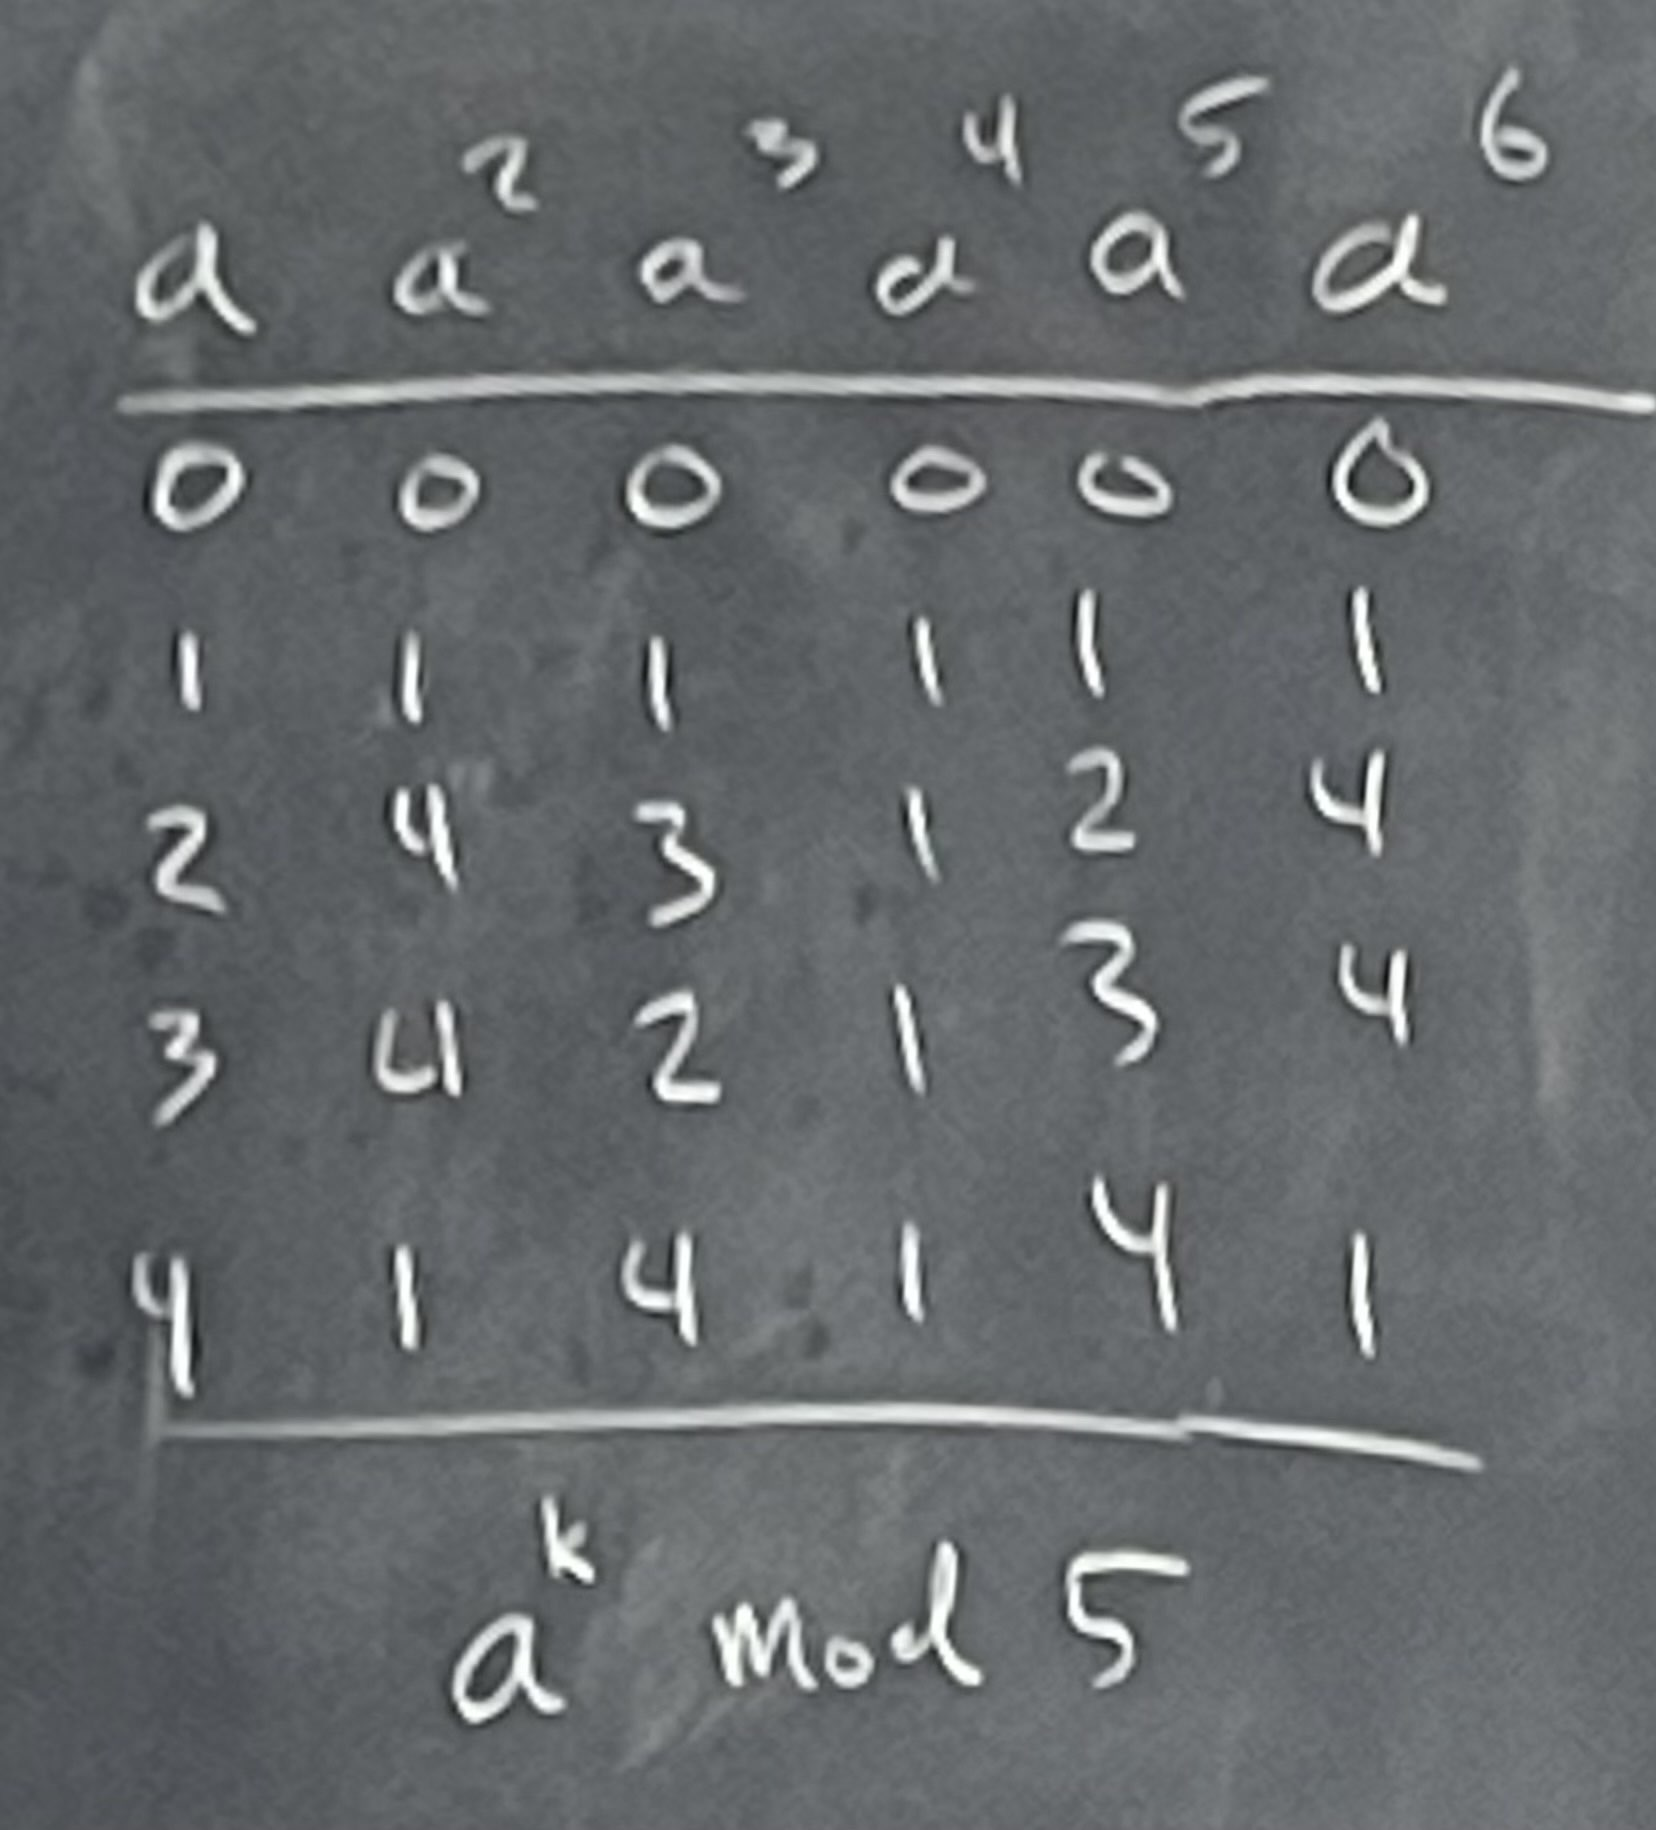
\includegraphics[scale=0.1]{Images/image1.jpg}\end{center}
    $a^k\pmod{7}$ \\
    \begin{center}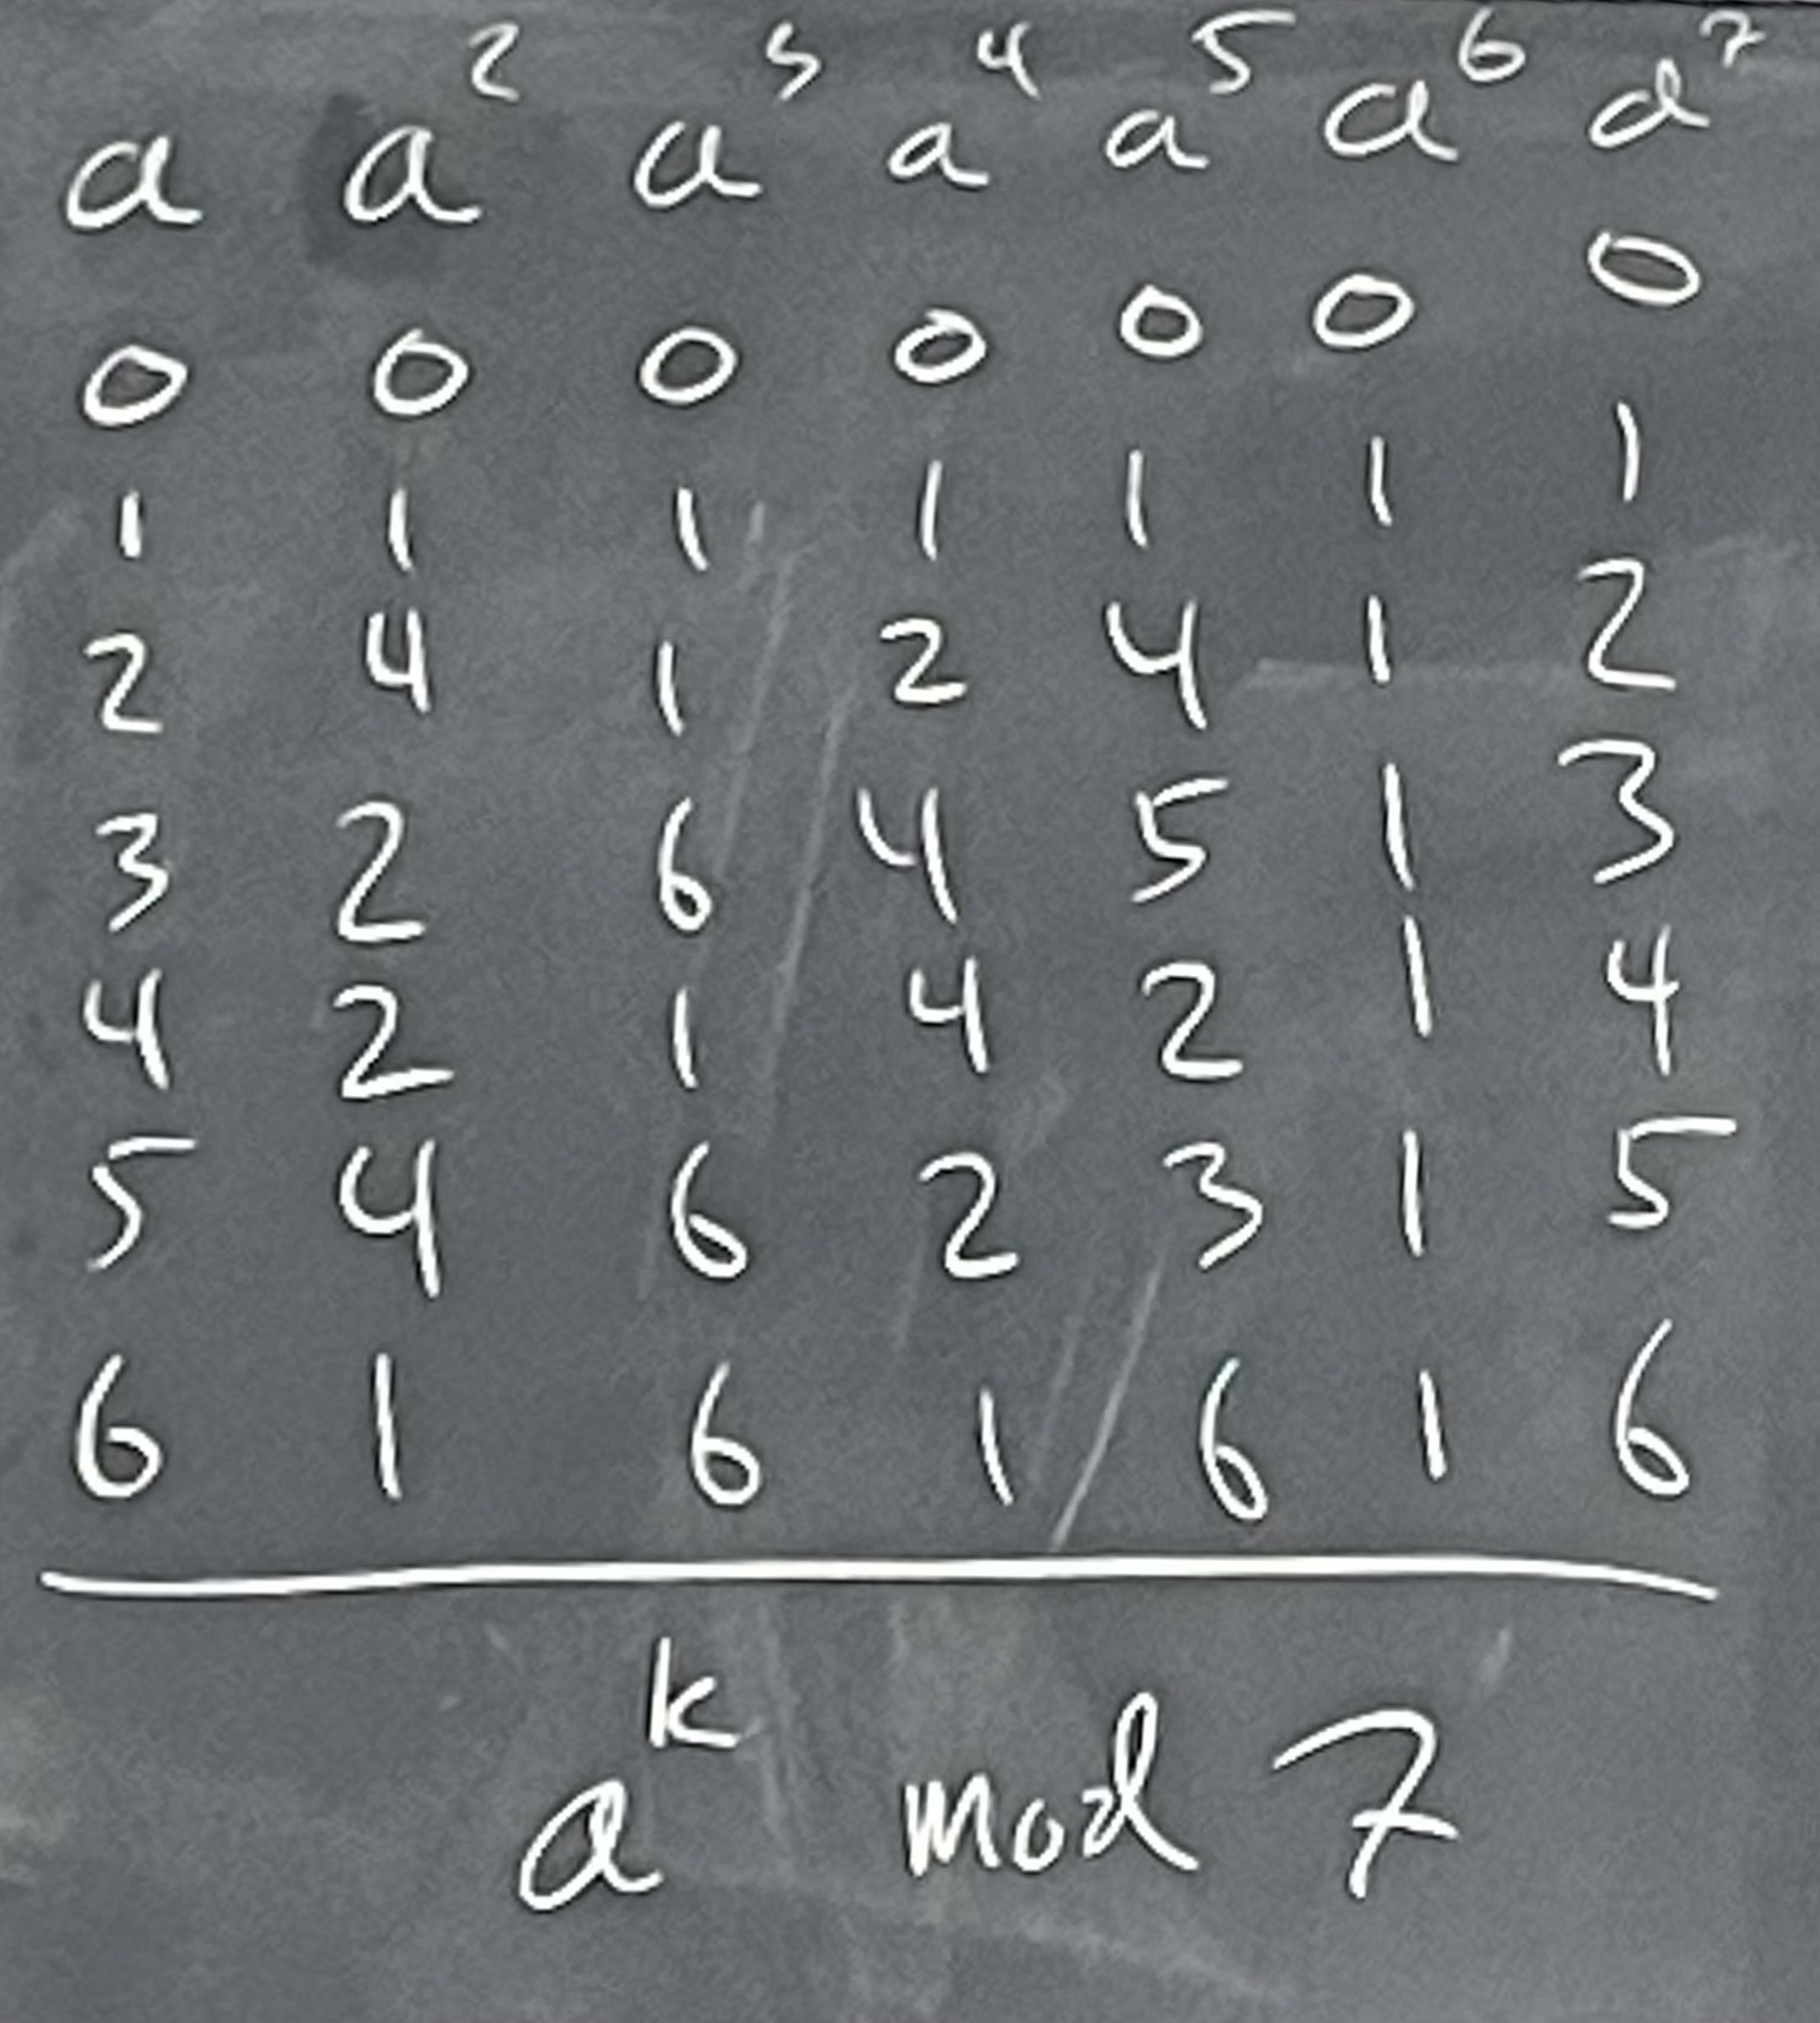
\includegraphics[scale=0.08]{Images/image2.jpg}\end{center}

    \subsection{Fermat's Little Theorem}
        \begin{theorem}
            Let $p$ be prime and $a\in\ZZ$ such that $p\nmid a$. Then
            \[
                a^{p-1}\equiv 1\pmod{p}
            \]
            ie.
            \[ 
                p\mid (a^{p-1}-1)
            \]
        \end{theorem}

        \begin{proof} [Proof (Idea)]
            $p=5$ 
            \begin{align*}
                0,1,2,3,4,5 \pmod{5} \\
                0,2,4,1,3 \pmod{5} \\
                0,3,1,4,2
            \end{align*}
        \end{proof}

        \underline{Claim}: The integers $0,a,2a,\dots, (p-1)a \pmod{p}$
        are the same as the integers $0,1,2,\dots,(p-1)$ but maybe
        in a different order.

        \begin{proof} [Proof of Claim]
            If claim is false, then $ia\equiv ja\pmod{p}$ for some $i,j$. 
            Then $p\mid a(i-j)$. \\
        \end{proof}

        Now Consider
        \begin{align*}
            & a(2a)(3a)\dots((p-1)(a)) \\
            &= a^{p-1}(1)(2)(3)\dots(p-1) \\
            &= a^{p-1}(p-1)!
        \end{align*}
        On the other hand, by the claim, 
        \begin{align*}
            a(2a)(3a)\dots((p-1)a) &\equiv (1)(2)(3)\dots(p-1) \pmod{p} \\
            a^{p-1}(p-1)! &\equiv (p-1)! \pmod{p}
        \end{align*}
        By HW, 
        \[ \gcd((p-1)!, p) = 1 \]
        So we can cancel: 
        \[ a^{p-1}\equiv 1\pmod{p} \]
        
    \subsection{Example}
            $p=23$. $6^{22}=1\pmod{23}$.  \\
            ie. \[ 23|(6^{22}-1) \]
        
    \subsection{Primality Test}
    $n=10^{100}+37$ \\
    Compute 
    \begin{align*} 
        2^{n-1} = 2^{10^{100}+36}\not\equiv 1\pmod{n} \\
        \equiv 367\dots 396\pmod{n}
    \end{align*}
    So n is \underline{not prime}. \\
    Note: This will \underline{never} show n is prime. It can be true that $a^{n-1}\equiv 1\pmod{n}$
    even if n is composite. \\
    Test 117 with $a=2$. 
    \begin{align*}
        2^{116} &= 2^{64}\cdot 2^{32}\cdot 2^{16}\cdot 2^{4} \\
        &\equiv 16\cdot 22 \cdot 16 \cdot 16 \\
        &\equiv 22 \\
        &\not\equiv 1\pmod{117}
    \end{align*}
    So 117 is composite.     

\documentclass[letterpaper]{article}

\usepackage{amssymb}
\usepackage{amsthm}
\usepackage{amsmath}
\usepackage[left=1in, right=1in, top=1in, bottom=1in]{geometry}

\newcommand{\ZZ}{\mathbb{Z}}
\newcommand{\NN}{\mathbb{N}}
\newcommand{\QQ}{\mathbb{Q}}

\newtheorem{lemma}{Lemma}
\newtheorem{sublemma}{Lemma}[lemma]
\newtheorem{theorem}{Theorem}[subsection]
\newtheorem{corollary}{Corollary}[subsection]
\newtheorem{definition}{Definition}[subsection]
\newtheorem{proposition}{Proposition}[subsection]
\newtheorem{example}{Example}[subsection]

\title{M 328K: Lecture 8}
\author{Katherine Ho}
\date\today

\begin{document}
\maketitle

\section{Last Time}
    \subsection{Fermat's Little Theorem}
        Let $p$ be prime, $a\in\ZZ$, $p\nmid a$, then 
        \[ a^{p-1}\equiv 1\pmod{p} \]
        \[ ax\equiv 1\pmod{n} \quad\text{has a solution whenever}\quad \gcd(a,n)=1 \]
        \begin{align*}
            4x &\equiv 3\pmod{19} \\
            4^{17}(4x) &\equiv 4^{17}\cdot 3\pmod{19} \\
            4^{18}x &\equiv 5\cdot 3\pmod{19} \\
            x &\equiv 15\pmod{19}
        \end{align*}
        \underline{Note}: Definitely need $p$ to be prime.
    \begin{example}
        \[ 3^9\equiv 3\pmod{10} \]
    \end{example}

\section{Generalization to composite modulus}
    \subsection{Euler Totient Function (Euler's Phi Function)}
    \begin{definition}
        The Euler totient function $\phi$ is 
        the function $\phi$ $\NN\rightarrow\NN$ defined by 
        \[ 
            \phi(n) = \#\{ a\mid 1\le a\le n-1, \gcd(a,n)=1 \} 
        \]
        \begin{example}
            \begin{align*}
                \phi(1) &= 1 \\
                \phi(2) &= 1 \\
                \phi(3) &= 2 \\
                \phi(4) &= 2 \\
                \phi(20) &= 8
            \end{align*}
        \end{example}

        \begin{proposition}
            If $p$ is prime, then
            \[ \phi(p) = p-1 \]
        \end{proposition}

        \begin{proposition}
            If $p$ is prime and $k>1$, then
            \[ \phi(p^k) = p^k-p^{k-1} \]
            Exclude all multiples of $p$ between 1 and $p^k$:
            \[ p,2p,3p,\dots,(p^{k-1})p,p^{k-1}p \]
        \end{proposition}

        \underline{Note}: $\phi(n)=n-1$ iff $n$ is prime.
        Intuition: $\phi$ is how close $n$ is to being prime.
    \end{definition}

    \subsection{Euler's Theorem}
    \begin{theorem} [Euler's Theorem]
        Let $\gcd(a,n)=1$. Then 
        \[ a^{\phi(n)}\equiv 1\pmod{n} \]
        Note: If $n=p$ is prime, then $\phi(n)=p-1$, so we get 
        \[ a^{p-1}\equiv 1\pmod{p} \]
        \begin{proof} [Proof of Euler's Theorem]
            Let $0<b_1<b_2<\dots<b_{\phi(n)}$ be the integers between 
            1 and $n$ that are coprime to $n$. The claim: The integers 
            $ab_1, ab_2, \dots, ab_{\phi(n)}$ are the same as 
            $b_1,b_2,\dots,b_{\phi(n)}\pmod{n}$ but maybe in a different order.
            \begin{example}
                $n=10$; $a-3$
                \[
                \begin{matrix}
                    b_1 & b_2 & b_3 & b_4 \\
                    1 & 3 & 7 & 9 \\
                    ab_1 & ab_2 & ab_3 & ab_4 & \pmod{10} \\
                    3 & 9 & 1 & 7
                \end{matrix}
                \]
                Proof is same from HW. \\
                So
                \begin{align*}
                    (ab_1)(ab_2) &\equiv b_1b_2\dots b_{\phi(n)} \pmod{n} \\
                    a^{\phi(n)}(b_1b_2\dots b_{\phi(n)}) &\equiv b_1b_2\dots b_{\phi(n)}
                \end{align*}
                Since each $b_i$ is coprime to $n$, we can cancel to get 
                \[ a^{\phi(n)}\equiv 1\pmod{n} \]
            \end{example}
        \end{proof}
    \end{theorem}

    \subsection{More on $\phi$}
        \begin{align*}
            \phi(p) &= p-1 \quad\text{for } p \text{ prime} \\
            \phi(p^k) &= p^k - p^{k-1} 
        \end{align*}

        \begin{theorem}
            Let $a,b$ be coprime positive integers. Then,
            \[ \phi(a,b)=\phi(a)\cdot\phi(b) \]
            "$\phi$ is multiplicative." \\\\
            \textbf{WARNING}: We need $\gcd(a,b)=1$.
            Ex. $\phi(4)=2$, $\phi(2)\phi(2)=1$
        \end{theorem}

        \begin{corollary}
            If $n=p_1^{r_1}\dots p_k^{r_k}$, then
            \[ 
                \phi(n) = \phi(p_1^{r_1})\dots\phi(p_k^{r_k})
                = (p^{r_1}-p^{r_{k-1}})\dots(p^{r_k}-p^{r_{k-1}})
            \]
        \end{corollary}

        To prove this, we first need to understand how to solve this 
        problem from 4th century China: 
        \begin{align*}
            x &\equiv 2\pmod{3} \\
            x &\equiv 3\pmod{5} \\
            x &\equiv 2\pmod{7}
        \end{align*}
        We will solve this using the \underline{Chinese Remainder Theorem}.

        \begin{theorem} [Chinese Remainder Theorem]
            Suppose $\gcd(n_1,n_2)=1$ for pos integers $n_1$ and $n_2$. 
            Then for any $a_1,a_2\in\ZZ$, the system
            \begin{align*}
                x\equiv a_1\pmod{n_1} \\
                x\equiv a_2\pmod{n_2}
            \end{align*} 
            has a unique solution $0\le x<n_1n_2$.

            \begin{proof} [Proof (Existence)]
                By Bezout, there exist $m_1,m_2\in\ZZ$ such that
                \[ n_1m_1+n_2m_2 = 1 \]
                Now let $x=a_2n_1m_1+a_1n_2m_2$.
                Then reducing $\pmod{n_1}$, we have
                \begin{align*}
                    x=a_2n_1m_1+a_1n_2m_2 &\equiv a_1n_2m_2\pmod{n_1} \\
                    &\equiv a_1(1-n_1m_1)\pmod{n-1} \\
                    &\equiv a_1-a_1n_1m_1\pmod{n-1} \\
                    &\equiv a_1\pmod{n_1}
                \end{align*}
                By the same argument, 
                \[ x\equiv a_2\pmod{n_2} \]
                Take $x\pmod{n_1n_2}$ to be a solution between 0 and $n_1n_2$.
            \end{proof}
        \end{theorem}

        \begin{example} 
            Going back to this problem, 
            \begin{align*}
                x &\equiv 2\pmod{3} \\
                x &\equiv 3\pmod{5} \\
                x &\equiv 2\pmod{7}
            \end{align*}
            First use Bezout:
            \begin{align*}
                3\cdot 2+5(-1)=1 \\
                x = 3(6)+2(-5)\pmod{15} = 8 \\
            \end{align*} 
            \begin{align*}
                x\equiv 8\pmod{15} \\
                x\equiv 2\pmod{7} \\
                15\cdot 1 + 7(-2) = 1 \\
                x = 2(15) + 8(-14)\pmod{105} \\
                -82\pmod{105} = 23
            \end{align*}
        \end{example}   

        \underline{Relationship with $\phi$}: To show
        \[ \phi(ab) = \phi(a)\phi(b) \]
        when $\gcd(a,b)=1$, we need to count two things: 
        \[ 
            \{ x\mid 0\le x<ab, \gcd(x,ab)=1 \} 
        \]
        \begin{center}Size: $\phi(ab)$\end{center}
        \[ 
            \{ (y_1,y_2)\mid 0\le y_1 < a, \gcd(y_1,a)=1,
            0\le y_2<b, \gcd(y_2,b)=1 \} 
        \]
        \begin{center}Size: $\phi(a)\phi(b)$\end{center}

\end{document}
\chapter{Lecture 9}
\date{September 24, 2024}

\section{Last Time}
    Chinese Remainder Theorem
    \begin{align*}
        x &\equiv a_1\pmod{n_1} \\
        x &\equiv a_2\pmod{n_2}
    \end{align*}
    has a unique solution mod $n_1n_2$. 
    \[ x\equiv\quad\text{a unique integer in}\quad 0,1,2,\dots,n_1n_2-1 \]
\chapter{Lecture 10}
\date{September 26, 2024}

\section{Some more properties of primes}
    \underline{Freshmen's Dream}
    \[ (x+y)^n = x^n + y^n \quad\text{False!} \]
    \begin{align*}
        (x+y)^n &= \sum_{k=0}^{n}x^k y^{n-k} \\
        \text{where}\quad {n\choose k} &= \frac{n!}{k!(n-k)!}
    \end{align*}
    If $n=p$ is prime, then
    \[ (x+y)^p = \sum_{k=0}^{p}{p\choose k}x^k y^{n-k} \]
    From HW: for $0<<k<p$, we have $p\mid {p\choose k}$. \\\\
    So, $(x+y)^p = x^p + y^p + p\cdot\text{some poly w/ } \ZZ \text{ coeffs}$. \\\\
    Reducing $\pmod{p}$, we have 
    \[ (x+y)^p\equiv x^p+y^p\pmod{p} \]

    On the topic of polynomials$\dots$ \\\\
    Solving $F(x)\equiv 0\pmod{n}$ can be weird. \\
    \begin{example}
        Find all solutions (up to congruence) to 
        \[ x^2\equiv 0\pmod{9} \]
        $x=0, x=3, x=6 \leftarrow 3$ roots to a polynomial $F(x)=x^2$ 
        of degree 2. \\
        This happens because 9 is not prime.
    \end{example}

    \begin{theorem}
        Let $F(x)$ be a polynomial of degree $r$. 
        Then $F(x)$ has at most $r$ roots mod any prime $p$
        (as long as $p\nmid$ (leading coeff)).
        \begin{example}
            From HW you showed that the only square roots of $1\pmod{p}$ 
            were 1 and -1.
        \end{example}
    \end{theorem}

\newpage
\section{Wilson's Theorem}
    \begin{theorem} [Wilson's Theorem]
        Let $p$ be a prime. Then
        \[ (p-1)!\equiv -1\pmod{p} \]
        \begin{example}
            $p=11$:
            \[ (1)(2)\dots(9)(10) \]
            \begin{itemize}
                \item 1 and 10 pair to themselves.
                \item 2 pairs with 6. $(2\cdot 6)-1$
                \item 3 pairs with 4.
                \item 5 pairs with 9.
                \item 7 pairs with 8.
            \end{itemize}
            \begin{align*}
                10! &= (1)(2\cdot 6)(3\cdot 4)(5\cdot 9)(7\cdot 8)\cdot 10 \\
                &\equiv (1)(1)(1)(1)(1)(-1) - 1 \pmod{11}
            \end{align*}
        \end{example}
        \begin{proof}
            Let $p$ be prime and consider the integers $2,3,\dots,p-2$.
            Each one of these integers has some inverse $\pmod{p}$.
            ie. If $a\in\{ 2,3,\dots,p-2 \}$, then $ax\equiv 1\pmod{p}$
            has a solution. \\\\
            Claim: For each $a\in\{ 2,3,\dots,p-2 \}$,
            \[ a\not\equiv a^{-1} \pmod{p} \]
            Why? If $a\equiv a^{-1}\pmod{p}$, then
            \[ a^2\equiv 1\pmod{p} \]
            From HW, the solutions are exactly 
            \[ a\equiv 1 \quad\text{or}\quad a\equiv -1 \]
            Then we can pair each $a\in\{ 2,3,\dots,p-2 \}$ with its inverse
            $\pmod{p}$ to get 
            \[ (p-1)! = 1((2)(3)\dots(p-2))(p-1) \equiv -1 \pmod{p} \]
            Note: $(2)(3)\dots(p-2)\equiv 1\pmod{p}$, $(p-1)\equiv -1\pmod{p}$.
        \end{proof}
        Note: We really need $p$ to be prime.
        \begin{example}
            Look at $x^2\equiv 1\pmod{8}$.
            \[ x\equiv 1, x\equiv -1(\equiv 7), x\equiv 3, x\equiv 5, x\equiv 7 \]
            Remark: $F(x) = x^2 - 1$ has 4 roots $\pmod{8}$. 
        \end{example}
    \end{theorem}

\newpage
\section{Review}
    \begin{example}
        Compute $3^{104}\pmod{101}$
        \begin{align*}
            3^{100} &\equiv 1\pmod{101} \\
            3^4\cdot 3^{100} &\equiv 3^4\pmod{101} \\
            3^{104} &\equiv 81\pmod{101}
        \end{align*}
    \end{example}

    \begin{example}
        For $n>3$, $\phi(n)$ is even. \\
        $\phi$ is multiplicative. $\rightarrow$ compute $\phi$ from prime factorization. \\
        Write $n=p_1^{k_1}\dots p_r^{k_r}$ then
        \[ \phi(n) = \phi(p_1^{k_1}\dots \phi(p_r^{k_r})) = (p_1^{k_1}-p_1^{k_1-1})\dots (p_r^{k_r} - p_r^{k_r-1}) \]

    \end{example}
\chapter{Lecture 11}
\date{October 3, 2024}

\section{}
\chapter{Lecture 12}
\date{October 8, 2024}

\section{Miscellaneous}
    \subsection{Least Common Multiple}
    \begin{definition}
        Let $a,b$ be positive integers. 
        The least common multiple of $a$ and $b$ denoted by 
        $\text{lcm}(a,b)$ is the smallest positive integer divisible by 
        $a$ and $b$. \\
        Examples
        \begin{itemize}
            \item $\text{lcm}(2,3)=6$
            \item $\text{lcm}(4,6)=12$
            \item $\text{lcm}(1,n)=n$
            \item $\text{lcm}(n,n)=n$
        \end{itemize}
        \[ 4\cdot 6 = 24, \gcd(4,6) = 2, \text{lcm}(4,6) = 12 \]
        \[ 3\cdot 9 = 27, \gcd(3,9) = 3, \text{lcm}(3,9) = 9 \]
        \begin{theorem}
            For positive integers $a,b$ we have 
            \[ ab = \gcd(a,b) \cdot \text{lcm}(a,b) \]
        \end{theorem}
    \end{definition}

    \subsection{More about $\phi$ (and number-theoretic functions)}
    \begin{definition}
        A number theoretic function (or arithmetic function) is a function
        \[ f: \NN \leftrightarrow \NN \quad(\text{or } \ZZ \leftrightarrow \ZZ) \]
        that has "number theory properties" \\
        Ex: 
        \begin{itemize}
            \item $\phi$
            \item $\tau(n) = \#$ of divisors of $n$
            \begin{align*}
                10:&\quad 1,2,5,10 \\
                \tau(10) &= 4 \\
                12:&\quad 1,2,3,4,6,12 \\
                \tau(12) &= 6
            \end{align*}
            \item  $\sigma(n) =$ \text{sum of divisors of n}
            \begin{align*}
                \sigma(10) &= 1 + 2 + 5 + 10 = 18 \\
                \sigma(12) &= 1+2+3+4+6+12=28
            \end{align*}            
        \end{itemize}
        Facts: $\phi,\tau,\sigma$ are all multiplicative.
        \begin{align*}
            \phi(ab) &= \phi(a)\phi(b) \\
            \sigma(ab) &= \sigma(a)\sigma(b) \quad\text{if } \gcd(a,b)=1\\
            \tau(ab) &= \tau(a)\tau(b)
        \end{align*}
        Notice: $\sigma(n) = \sum_{d\mid n}^{}d, \quad\tau(n) = \sum_{d\mid n}^{}1$ \\
        ($d\mid n$ is sum over positive divisors of $n$)        
    \end{definition}
    \begin{example}
        Define $F(n) = \sum_{d\mid n}^{}\phi(d)$
        \begin{align*}
            F(12) &= \sum_{d\mid 12}^{}\phi(d) \\
            &= \phi(1)+\phi(2)+\phi(3)+\phi(4)+\phi(6)\phi(12) \\
            &= 1+1+2+2+2+4 \\
            F(12) &= 12
        \end{align*}
        \begin{align*}
            F(15) &= \phi(1)+\phi(3)+\phi(5)\phi(15) \\
            &= 1+2+4+8 \\
            F(15) &= 15
        \end{align*}
    \end{example}
    \begin{theorem}
        For all pos  integers $n$,
        \[ n = \sum_{d\mid n}^{}\phi(d) \]
        \begin{proof}
            (Step 1) Lemma: If $f: \NN\leftrightarrow\NN$ is multiplicative, 
            then the function 
            \[ F(n) = \sum_{d\mid n}^{}f(d) \]
            is multiplicative. (Proof: HW) \\\\
            (Step 2) We know that $F(n) = \sum_{d\mid n}^{}\phi(d)$
            is multiplicative, since $\phi$ is multiplicative. \\
            Lets show $F(n)=n$ for primes and prime powers. \\
            If $p$ is prime, then $F(p) = \sum_{d\mid p}^{}\phi(d)
            = \phi(1) + \phi(p) = 1 + (p-1) = p$ \\
            Now calculate for $k\ge 1$
            \begin{align*}
                F(p^k) &= \sum_{d|p^k}^{}\phi(d) \\
                &= \phi(1) + \phi(p) + \phi(p^2) + \dots + \phi(p^k) \\
                &= 1 + (p-1) + (p^2-p) + \dots + (p^j-p^{j-1})+(p^k-p^{k-1}) \\
                F(p^k) &= p^k
            \end{align*}
            Now let $n=p_1^{k_1}\dots p_r^{k_r}$
            \begin{align*}
                F(n) &= F(p_1^{k_1})\dots F(p_r^{k_r}) \\
                &= p_1^{k_1}\dots p_r^{k_r} \\
                &= n
            \end{align*}
        \end{proof}
    \end{theorem}

    \subsection{Lagrange's Theorem}
    Recall $x^2\equiv 1\pmod{8}$ has $x\equiv 1,3,5,7$ (4 solutions). But\dots
    \begin{theorem} [Lagrange's Theorem]
        Let $f(x)$ be a polynomial of degree $d$ with integer coefficient
        and $p$ be prime. Suppose $p\nmid $(leading coefficient). \\
        Then $f(x)\equiv 0\pmod{p}$ has at most $d$ incongruent solutions.
        \begin{proof} 
            By induction on the degree d. \\
            Base case: $d=1$, $f(x) = a_1x+a_o$ and $p\nmid a_1$. 
            Then 
            \begin{align*}
                f(x) &\equiv 0\pmod{p} \\
                a_1x+a_0 &\equiv 0\pmod{p} \\
                a_1x &\equiv a_0\pmod{p}
            \end{align*}
            has a unique solution since $\gcd(a_1,p) = 1\le d$. \\\\
            Induction step: Let's assume the statement is true for all 
            polynomials of degree $\le k$. \\
            Now let 
            $f(x)\equiv a_{k+1}x^{k+1}+\dots+a_1x+a_0$ where $p\nmid a_{k+1}$.
            If $f(x)\equiv 0\pmod{p}$ has no solutions, then we are done since
            $0<k+1$. Hence suppose $x=a$ is a solution. \\
            By the division algorithm applied to $f(x)$ and $x-a$, we have
            \begin{align*}
                f(x) &= (x-a)\cdot q(x) + r, \quad r\in\ZZ  \\
                f(a) &\equiv 0\pmod{p} \\
                r &\equiv 0\pmod{p}
            \end{align*}
            Thus, $f(x)\equiv (x-a)\cdot q(x)\pmod{p}$. By IH, $q(x)\equiv 0\pmod{p}$
            has at most k solutions. Thus $f(x)\equiv 0\pmod{p}$ has at most $k+1$ solutions. \\
        \end{proof}
    \end{theorem}

\section{Order}
    \subsection{}
    \begin{definition}
        Let $\gcd(a,n)=1$. Then the smallest positive integer $k$ such that
        $a^k\equiv 1\pmod{n}$ is called the order of a modulo n and is denoted by 
        $\text{ord}_n(a)$ or just $\text{ord}(a)$ is it's unambiguous.
    \end{definition}
    \begin{example}
        $a^k\pmod{7}$
    \end{example}
    \begin{theorem}
        Suppose $\gcd(a,n)=1$ and $a^k\equiv 1\pmod{n}$. Then ord$(a)\mid k$.
        \begin{proof}
            By division algorithm, write
            \[ k = \text{ord}(a)\cdot q + r, \quad 0\le r<\text{ord}(a) \]
            Then 
            \begin{align*}
                a^k &\equiv 1\pmod{n} \\
                a^{\text{ord}(a)\cdot q}\cdot a^r &\equiv 1\pmod{n} \\
                a^{\text{ord}(a)^q}\cdot a^r &\equiv 1\pmod{n} \\
                a^r &\equiv 1\pmod{n}
            \end{align*}
            Then $r=0$, otherwise r is a smaller exponent for $a^r\equiv 1\pmod{n}$
            contradicting ord$(a)$ being the smallest. 
            Thus $k=$ ord$(a)\cdot q$ so ord$(a)\mid k$.
        \end{proof}
    \end{theorem}
\chapter{Lecture 13}
\date{October 10, 2024}

\section{}
\chapter{Lecture 14}
\date{October 15, 2024}

\section{Recap}
    If $\gcd(a,n) = 1$, the order of $a$ is the smallest positive exponent
    $k$ such that $a^k\equiv 1\pmod{n}$
    \begin{itemize}
        \item If $a^m\equiv 1\pmod{n}$, then $\ord{a}\mid m$
        \item $a,a^n,\dots,a^{\ord{n}}$ are all incongruent $\pmod{n}$
        \item If $\ord{a}=\phi(n)$, then $a$ is called a \underline{primitive root} and
        $a,\dots,a^{\phi(n)}\pmod{n}$ are congruent to all the integers between $1$ and $n$, 
        coprime to $n$
    \end{itemize}

\section{All primes have a primitive root}
    \begin{theorem}
        Let $p$ be prime and $d\mid p-1$. Then there are exactly $\phi(d)$
        integers (that are mutually incongruent $\pmod{p}$) that have
        order $d\pmod{p}$. In particular there are $\phi(p-1)$ primitive roots.
        \begin{lemma}
            If $d\mid p-1$, then $x^d\equiv 1\pmod{p}$ has exactly $d$ incongruent
            solutions $pmod{p}$.
            \begin{proof}
                $x^{p-1}-1\equiv x^{dk}-1 = (x^d - 1)(x^{d(k-1)}+\dots+x^d+x)$
            \end{proof}
        \end{lemma}
        \begin{proof} [Proof of Thm.]
            Define $\psi(d) = \#$ of integers $1\le x\le p-1$ having order $d\pmod{p}$. \\

            \underline{WTS}: $\psi(d) = \phi(d)$ for $d\mid p-1$ \\
            Instead, let's prove $\psi(d)\le \phi(d)$ when $d\mid p-1$. 
            If there are no integers with order $d$, then
            \[ \psi(d) = 0\le \phi(d) \]
            Hence assume there exists at least one integer $a$ with $\ord_{p}{a} = d$. \\

            \underline{Claim}: If $b$ has order $d$, then $b\equiv a^h\pmod{p}$ for some $h$.
            Why? If $b$ has order $d$, then $b$ satisfies:
            \[ x^d\equiv 1\pmod{p} \quad*\]
            which has exactly $d$ incongruent solutions. On the other hand,
            the integers $a,a^2,a^3,\dots,a^d$ are all incongruent $\pmod{p}$
            and they all satisfy $*$, since 
            \[ (a^{i})^d \equiv (a^d)^i \equiv 1^i \equiv 1 \pmod{p} \]
            Since $*$ has exactly $d$ solutions $\pmod{p}$, we must have 
            $b\equiv a^h\pmod{p}$ for some $h$, $1\le h\le d$. \\

            Now, we need to determine which $a^k$ has $\ord{a^k} = d$. 
            But $\ord{a^k} = \frac{d}{\gcd(h,d) = d}$
            precisely when $\gcd(h,d) = 1$. Hence there are exactly
            $\phi(d)$ exponents $h$ such that $a^h$ has order $d$. 
            Thus, we find $\psi(d)=\phi(d)$. We have shown for $d\mid p-1$,
            $\psi(d)$ is either $0$ or $\phi(d)$. But we know $\psi(d)\le \phi(d)$.

            Consider the sum
            \[ \sum_{d\mid p-1}^{}\psi(d). \]
            Note every integer $a$ between $1\le a\le p-1$ has some $\ord{a}$ 
            that divides $p-1$.
            Since each integer between $1$ and $p-1$ is counted exactly once,
            we have 
            \[ \sum_{d\mid p-1}^{} \psi(d) = p-1 \]
            \begin{mdframed}
            \begin{example}
                p = 7 
                \begin{align*}
                    \ord{1} &= 2 \\
                    \ord{2} &= 3 \\
                    \ord{3} &= 6 \\
                    \ord{4} &= 3 \\
                    \ord{5} &= 6 \\
                    \ord{6} &= 2
                \end{align*}
                \begin{align*}
                    \sum_{d\mid p-1}^{}\psi(d) &= \sum_{d\mid 6}^{} \psi(d) \\
                    &= \psi(1)+\psi(2)+\psi(3)+\psi(6) \\
                    &= 1+1+2+2 \\
                    &= 6 \\
                    &= p-1
                \end{align*}
            \end{example}
            \end{mdframed}

            Recall 
            \[ \sum_{d\mid p-1}^{}\phi(d) = p-1 \]
            Hence
            \[ \sum_{d\mid p-1}^{}\psi(d) = \sum_{d\mid p-1}^{}\phi(d), \quad\psi(d)\le \phi(d) \]  
            Thus $\psi(d) = \phi(d) \quad\forall\quad d\mid p-1$.
        \end{proof}
    \end{theorem}

    \underline{Note}: Once you have a primitive root $g$, then all the other primitive roots
    are congruent to $g^h$ where $\gcd(h,p-1) = 1$.

\section{How to find a primitive root}
    \begin{definition}
        Let $g$ be a primitive root of $p$ (or $n$ if $n$ has a primitive root).
        If $1\le a\le p-1$, the smallest positive exponent $k$ with $a\equiv g^k\pmod{p}$
        is called the \underline{index of $a\pmod{p}$} relative to $g$, 
        denoted $\ind(a)$.
    \end{definition}

\end{document}